\documentclass[
  russian,
  aspectratio=169,
  xcolor={svgnames},
  hyperref={colorlinks,citecolor=DeepPink4,linkcolor=DarkRed,urlcolor=DarkBlue}]{beamer}
\beamertemplatenavigationsymbolsempty % remove navigation bar
% \setbeamertemplate{headline}  % remove heading

\usetheme{Madrid}
% \usetheme{Warsaw}
\usecolortheme{beaver}


% \makeatletter
% \def\th@mystyle{%
%     \normalfont % body font
%     \setbeamercolor{block title example}{bg=blue,fg=white}
% %     \setbeamercolor{block body example}{bg=orange!20,fg=black}
%     \def\inserttheoremblockenv{exampleblock}
%   }
% \makeatother
% \theoremstyle{mystyle}

\makeatletter
\@ifclassloaded{beamer}{
  % get rid of header navigation bar
  \setbeamertemplate{headline}{}
  % get rid of bottom navigation symbols
  \setbeamertemplate{navigation symbols}{}
  % get rid of footer
  %\setbeamertemplate{footline}{}
}
{}
\makeatother
%%%%%%%%%%%%%%%%%%%%%%%%%%%%%%%%%%%%%%%%%%%%%
\usepackage{fontawesome}
% \newfontfamily{\FA}{Font Awesome 5 Free} % some glyphs missing
\expandafter\def\csname faicon@facebook\endcsname{{\FA\symbol{"F09A}}}
\def\faQuestionSign{{\FA\symbol{"F059}}}
\def\faQuestion{{\FA\symbol{"F128}}}
\def\faExclamation{{\FA\symbol{"F12A}}}
\def\faUploadAlt{{\FA\symbol{"F093}}}
\def\faLemon{{\FA\symbol{"F094}}}
\def\faPhone{{\FA\symbol{"F095}}}
\def\faCheckEmpty{{\FA\symbol{"F096}}}
\def\faBookmarkEmpty{{\FA\symbol{"F097}}}

\newcommand{\faGood}{\textcolor{ForestGreen}{\faThumbsUp}}
\newcommand{\faBad}{\textcolor{red}{\faThumbsODown}}
\newcommand{\faWrong}{\textcolor{red}{\faTimes}}
\newcommand{\faMaybe}{\textcolor{blue}{\faQuestion}}
\newcommand{\faCheckGreen}{\textcolor{ForestGreen}{\faCheck}}
%%%%%%%%%%%%%%%%%%%%%%%%%%%%%%%%%%%%%%%%%%%%%

\usepackage{fontspec}
\usepackage{xunicode}
\usepackage{xltxtra}
\usepackage{xecyr}
\usepackage{hyperref}

\setmainfont[
 Ligatures=TeX,
 Extension=.otf,
 BoldFont=cmunbx,
 ItalicFont=cmunti,
 BoldItalicFont=cmunbi,
% Scale = 1.1
]{cmunrm}
\setsansfont[
 Ligatures=TeX,
 Extension=.otf,
 BoldFont=cmunsx,
 ItalicFont=cmunsi,
%  Scale = 1.2
]{cmunss}
%\setmainfont[Mapping=tex-text]{DejaVu Serif}
%\setsansfont[Mapping=tex-text]{DejaVu Sans}
%\setmonofont{Fira Code}[Contextuals=AlternateOff]
\setmonofont{Fira Code}[Contextuals=Alternate,Scale=0.9]
\newfontfamily{\myfiracode}[Scale=1.5,Contextuals=Alternate]{Fira Code}
%\setmonofont[Scale=0.9,BoldFont={Inconsolata Bold}]{Inconsolata}

\usepackage{polyglossia}
\setmainlanguage{russian}
\setotherlanguage{english}


%\newfontfamily\dejaVuSansMono{DejaVu Sans Mono}
% https://github.com/vjpr/monaco-bold/raw/master/MonacoB/MonacoB.otf
%\newfontfamily\monacoB{MonacoB}
%%%%%%%%%%%%%%%%%%%%%%%%%%%%%%%%%%%%%%%%%%%%%%%5
\usepackage{soul} % for \st that strikes through
\usepackage[normalem]{ulem} % \sout

\usepackage{stmaryrd}
\newcommand{\sem}[1]{\ensuremath{\llbracket #1\rrbracket}}


\usepackage{listings}
%\lstdefinestyle{style1}{
%  language=haskell,
%  numbers=left,
%  stepnumber=1,
%  numbersep=10pt,
%  tabsize=4,
%  showspaces=false,
%  showstringspaces=false
%}
%\lstdefinestyle{hsstyle1}
%{ language=haskell
%%          , basicstyle=\monacoB
%         , deletekeywords={Int,Float,String,List,Void}
%         , breaklines=true
%         , columns=fullflexible
%         , commentstyle=\color{ForestGreen}
%         , escapeinside=§§
%         , escapebegin=\begin{russian}\commentfont
%         , escapeend=\end{russian}
%         , commentstyle=\color{ForestGreen}
%         , escapeinside=§§
%         , escapebegin=\begin{russian}\color{ForestGreen}
%         , escapeend=\end{russian}
%         , mathescape=true
%%          , backgroundcolor = \color{MyBackground}
%}
%
%\newcommand{\inline}[1]{\lstinline{haskell}{#1}}
%\def\hsinline{\mintinline{haskell}}
%\def\inline{\hsinline}
%
%\lstnewenvironment{hslisting} {
%    \lstset { style={hsstyle1} }
%  }
%  {}
%  
%%%%%%%%%%%%%%%%%%%%%%%%%%%%%%%%%%%%%%%%%%%%%%%%%%%%%%%%%%%  
%%\setmainfont[
%% Ligatures=TeX,
%% Extension=.otf,
%% BoldFont=cmunbx,
%% ItalicFont=cmunti,
%% BoldItalicFont=cmunbi,
%%]{cmunrm}
%%% С засечками (для заголовков)
%%\setsansfont[
%% Ligatures=TeX,
%% Extension=.otf,
%% BoldFont=cmunsx,
%% ItalicFont=cmunsi,
%%]{cmunss}
%% \setmonofont[Scale=0.6]{Monaco}
%
%\usefonttheme{professionalfonts}
%\usepackage{times}
\usepackage{tikz}
\usetikzlibrary{cd}
\usepackage{tikz-cd}
\usepackage{caption}
\usepackage{subcaption}

%\renewtheorem{definition}{برهان}[chapter]
%%\DeclareMathOperator{->}{\rightarrow}
%\newcommand\iso{\ensuremath{\cong}}
%\usepackage{verbatim}
%\usepackage{graphicx}
%\usetikzlibrary{arrows,shapes}

%\usepackage{amsmath}
%\usepackage{amsfonts}
\usepackage{scalerel}
\DeclareMathOperator*{\myvee}{\scalerel*{\vee}{\sum}}
\DeclareMathOperator*{\mywedge}{\scalerel*{\wedge}{\sum}}

%
%\usepackage{tabulary}
%
%% sudo aptget install ttf-mscorefonts-installer
%%\setmainfont{Times New Roman}
%%\setsansfont[Mapping=tex-text]{DejaVu Sans}
%
%%\setmonofont[Scale=1.0,
%%    BoldFont=lmmonolt10-bold.otf,
%%    ItalicFont=lmmono10-italic.otf,
%%    BoldItalicFont=lmmonoproplt10-boldoblique.otf
%%]{lmmono9-regular.otf}
%
\usepackage[cache=true]{minted}
\usemintedstyle{perldoc}

\def\hsinline{\mintinline{haskell}}
\def\mlinline{\mintinline{ocaml}}
% color options
\definecolor{YellowGreen} {HTML}{B5C28C}
\definecolor{ForestGreen} {HTML}{009B55}
\definecolor{MyBackground}{HTML}{F0EDAA}



\institute{матмех СПбГУ}

\addtobeamertemplate{title page}{}{
  \begin{center}{\tiny Дата сборки: \today}\end{center}
}


\usepackage{subcaption}
\newtheorem{thm}{Theorem}
% \newtheorem*{remark}{Remark}

\newcommand{\naturalto}{%
  \mathrel{\vbox{\offinterlineskip
    \mathsurround=0pt
    \ialign{\hfil##\hfil\cr
      \normalfont\scalebox{1.5}{.}\cr
      \noalign{\kern-.15ex}
      $\longrightarrow$\cr}
  }}%
}


\title{Лемма Йонеды}
\author[Косарев Дмитрий]{Косарев Дмитрий a.k.a. Kakadu}

\institute[]{матмех СПбГУ}

\date{\today}

\AtBeginSection[]
{
  \begin{frame}<beamer>
    \frametitle{Содержание}
    \tableofcontents[currentsection,currentsubsection]
  \end{frame}
}

\newcommand{\verbatimfont}[1]{\def\verbatim@font{#1}}
\usepackage{verbatimbox}

\usepackage{amssymb,amsmath}
\usepackage{tikz}
\usepackage{tikz-cd}
\usetikzlibrary{arrows}
\tikzstyle{line}=[draw] % here
\tikzstyle{startstop} = [rectangle, rounded corners, minimum width=3cm,
    minimum height=1cm,text centered, draw=black, fill=red!30]
\usetikzlibrary{babel}


\begin{document}
\maketitle

% For every picture that defines or uses external nodes, you'll have to
% apply the 'remember picture' style. To avoid some typing, we'll apply
% the style to all pictures.
\tikzstyle{every picture}+=[remember picture]

% By default all math in TikZ nodes are set in inline mode. Change this to
% displaystyle so that we don't get small fractions.
\everymath{\displaystyle}

% Uncomment these lines for an automatically generated outline.
% \begin{frame}{Outline}
%   \tableofcontents
% \end{frame}

\section{Предварительные знания о терии категорий}

\begin{frame}[fragile]{Категории}
 Категория $\mathbb{C}$ состоит из:
\begin{itemize}
 \item набора \textit{объектов} |$\mathbb{C}$|;
 \item множества \textit{стрелок} $\mathbb{C}(A, B)$ из объекта $A$ в объект $B$ (идексированное парами объектов $A, B \in |\mathbb{C}|$);
 \item тождественная (identity) стрелка $id_A \in\mathbb{C}(A, A)$ для каждого объекта $A \in |\mathbb{C}|$;
 \item композиций $g\circ f \in\mathbb{C}(A, C)$ для каждой пары ``соединяемых'' стрелок $f \in\mathbb{C}(A, B)$ and $g \in\mathbb{C}(B, C)$,\\
\end{itemize}
и такая, что 
\begin{itemize}
 \item композиция ассоциативна;
 \item соответсвующие тождественные стрелки служат нейтральными элементами для композиции.
\end{itemize}
\vspace{0.5cm}
Стрелки ещё называют \textit{морфизмами}.
\end{frame}

\begin{frame}[fragile]{Локально малые (locally small) категории}
\begin{definition}
\emph{Локально малая} категория -- у которой набор стрелок между двумя произвольными объектами образует множество.
\end{definition}
\begin{definition}
\emph{Малая} категория -- это локально малая категория, у которой набор \emph{объектов} образует множество.
\end{definition}
\vspace{1cm}
Наборы стрелок в категории $\mathbb{C}$ из объекта A в объект B обозначаются $\mathbb{C}(A, B)$.

Множества $\mathbb{C}(A, B)$ называются homsets. 
\end{frame}

\begin{frame}[fragile]{Примеры}
Категория $\mathbb{S}et$ локально малая
\begin{itemize}
 \item Объекты -- множества
 \item Стрелки из $\mathbb{S}et(A,B)$ -- всюду определенные отображения из $A$ в $B$
\end{itemize}
\vspace{1cm}

На типы и программы можно смотреть как на категорию $\mathbb{H}ask$. 

Тогда объекты будут типами, а стрелки -- программами.
\end{frame}

\begin{frame}[fragile]{Примеры}
Любой предпорядок на множестве $(A,\leqslant)$ порождает категорию  $\mathbb{P}re(A,\leqslant)$

\begin{itemize}
 \item Объекты -- элементы множества A
 \item Множества homset $\mathbb{P}re(A,\leqslant)(a,b)$ 
    \begin{itemize}
    \item либо состоят из одного элемента (когда $a\leqslant b$)
    \item либо пустые
    \end{itemize}
\end{itemize}
\vspace{1cm}
Рефлексивность $a\leqslant a$ соответствует $id_a$.

Транзитивность -- это композиция стрелок.
\end{frame}

\begin{frame}[fragile]{Примеры}
\begin{minipage}{0.65\textwidth}
Всякий моноид $(M,\oplus,e)$ порождает категорию 
$\mathbb{M}on(M,\oplus,e)$

\begin{itemize}
 \item С единственным объектом $*$
 \item C единственным homset $\mathbb{M}on(M,\oplus,e)(*,*)$ 
    \begin{itemize}
    \item нейтральный элемент отображается в identity стрелку
    \item остальные элементы -- в остальные стрелки
    \end{itemize}
\end{itemize}
\vspace{1cm}
\end{minipage}
\begin{minipage}{0.3\textwidth}
 \begin{tikzpicture}
  \draw[thick, ->] (7,2) arc (0:360:1cm);% syntax (starting point coordinates) arc (starting angle:ending angle:radius)
  \draw[thick, ->] (7,2) arc (0:360:0.5cm);
  \draw[thick, ->] (7,2) arc (0:360:1.5cm);
  \draw[black,fill=black] (7,2.1) circle (.5ex); 
 \end{tikzpicture}
 
\end{minipage}

%%%%%%%%%%%%%%%%%%%%%%%%%%%%% 


\end{frame}

\begin{frame}[fragile]{Дуальная (двойственная, opposite) категория}
У каждой категории $\mathbb{C}$ есть \emph{дуальная} категория $\mathbb{C}^{op}$ с теми же объектами и развернутыми стрелками
\begin{itemize}
 \item объекты $\mathbb{C}^{op}$ -- это объекты $\mathbb{C}$, и наоборот;
 \item стрелки $\mathbb{C}^{op}(A,B)$ из $A$ в $B$ категории $\mathbb{C}^{op}$
 являются стрелками $\mathbb{C}(B,A)$ из $B$ в $A$ категории $\mathbb{C}$;
 \item композиция направлена в обратную сторону
\end{itemize}

\vspace{1cm}

TODO: рассказать про дуальность.
\end{frame}
% 
% \begin{frame}[fragile]{Произведение категорий}
% Для категорий $\mathbb{C}$ и $\mathbb{D}$, категория произведений $\mathbb{C}\times\mathbb{D}$ состоит из пар объектов и пар стрелок:
% 
% \begin{itemize}
%  \item  объекст $(A, B) \in |C × D|$ для каждой пары объектов $A \in |\mathbb{C}|$ and $B \in |\mathbb{D}|$;
% \item  стрелка $(f,g) \in (\mathbb{C}\times\mathbb{D})((A, B), (C, D))$ для каждой пары стрелок  
% $f\in \mathbb{C}(A, C)$ and $g \in \mathbb{D}(B, D)$;
% \item композиция задается поточечно.
% \end{itemize}
% \end{frame}

\begin{frame}[fragile]{TODO: про декартову замкнутость}

 И на примере Haskell тоже
 
\end{frame}

\begin{frame}[fragile]{Функторы}
Функторы -- это отображения между категориями, сохраняющие структуру.
\vspace{1cm}

Формально, функтор $F: \mathbb{C} \rightarrow \mathbb{D}$ -- это отображение объектов и стрелок из $\mathbb{C}$ в объекты и стрелки из $\mathbb{D}$, такое, что 
\begin{itemize}
 \item объект $F(A) \in |\mathbb{D}|$ для каждого объекта $A \in |\mathbb{C}|$;
 \item стрелка $F(f) \in \mathbb{D}(F(A), F(B))$ для каждой стрелки 
$f \in\mathbb{C}(A, B)$,
 \item $F(id_A ) = id_{F(A)}$ для каждого объекта $A \in |\mathbb{C}|$;
 \item $F (g \circ f) = F (g) \circ F (f)$ для каждой пары $f$ , $g$ ``соединяемых'' стрелок.
\end{itemize}

TODO: сказать про категорию (малых) категорий, что там стрелки -- это функторы, а объекты -- малые категории. И свойства программерского функутора вытекают из свойств стрелок.
\end{frame}

\begin{frame}[fragile]{Homfunctor}
Дана $\mathbb{C}$ и объекты $A,B \in |\mathbb{C}|$, homset $\mathbb{C}(A, B)$ -- это множество стрелок; \vspace{0.5cm}

Введем $\mathbb{C}(A, −)$ -- это отображение из $|\mathbb{C}|$ в $|\mathbb{S}et|$, переводящее объекты $B \mapsto\mathbb{C}(A, B)$ (т.е. объекты в набор морфизмов). \vspace{0.5cm}

Его можно расширить до стрелок $f \in \mathbb{C}(B, C)$:\\
$f \mapsto (f \circ) \in \mathbb{S}et(\mathbb{C}(A, B), \mathbb{C}(A, C))$
\vspace{0.5cm}

Функтор $\mathbb{C}(A, −)$ из $\mathbb{C}$ в $\mathbb{S}et$ будем называть \textit{homfunctor}. \vspace{0.5cm}

Аналогично, $\mathbb{C}(−, B)$ функтор преобразующий $f\mapsto(\circ f)$; но контравариантный, т.е. homfunctor из категории $\mathbb{C}^{op}$ в 
$\mathbb{S}et$

\end{frame}

\begin{frame}[fragile]
\begin{figure}
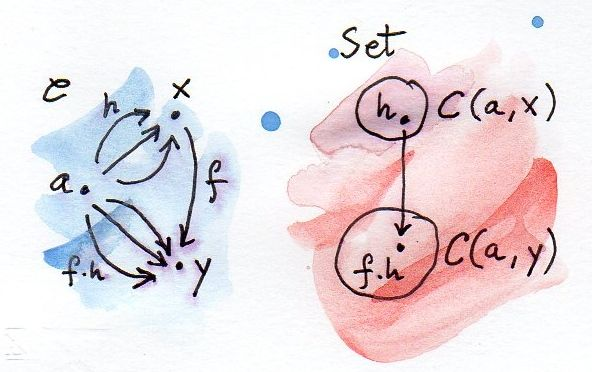
\includegraphics{hom-functor.jpg}
\caption{Ковариантный Hom функтор от \href{https://bartoszmilewski.files.wordpress.com/2015/07/hom-functor.jpg}{Бартоша Милевски}}
\end{figure}

% Тут мы сиспользхуем функтор, а не оперирует термином стрелка, потому что категория множест локально 
% малая и не понятно как быдут выглядеть стрелки в неё. И непонятно, что это за категория, которая 
% содержит локально малые категории, да и говорить об этом не хочется.

\end{frame}

\begin{frame}[fragile]{В терминах Haskell}
Ковариантный -- композиция после
\begin{hslisting}
type Reader a x = a -> x

instance Functor (Reader a) where
    fmap f h = f . h 
\end{hslisting}
Контравариантный -- композиция до
\begin{hslisting}
type Op a x = x -> a

instance Contravariant (Op a) where
    contramap f h = h . f
\end{hslisting}

\end{frame}



\begin{frame}[fragile]{Примеры функторов}
Функторы $\mathbb{P}re(A, \leqslant) \rightarrow \mathbb{P}re(B, \sqsubseteq)$ -- это монотонные функции
\vspace{1cm}

Функторы $\mathbb{M}on(M, \oplus, e) \rightarrow \mathbb{M}on(N, \otimes, e^{\prime})$ -- гомоморфизмы моноидов


% Функтор $F: \mathbb{M}on(M, \oplus, e) \rightarrow \mathbb{S}et$ ????????

\end{frame}


\begin{frame}[fragile]{Естественные преобразования (natural transformations)}
По сути: отображение между функторами, сохраняющее структуру.\vspace{0.4cm}

Формально, даны функторы $F,G : \mathbb{C} \rightarrow \mathbb{D}$. \textit{Естественным преобразованием} 
$\phi : F \overset{\text{\normalsize .}}\longrightarrow G$ из $F$ в $G$ будет 
семейство стрелок в $\mathbb{D}$ индексированное объектами из $\mathbb{C}$, такое что
\begin{itemize}
 \item стрелка $\phi_{A} \in \mathbb{D}(F(A), G(A))$ для каждого объекта
 $A \in |\mathbb{C}|$;
 \item \textit{условие натуральности}: для произвольной стрелки $f \in \mathbb{C}(A, B)$ верно $\phi_{B} \circ F(f)=G(f) \circ \phi_{A}$ 
\end{itemize}
\begin{tikzpicture}
  \matrix (m) [matrix of math nodes,row sep=2em,column sep=2em,minimum width=1em]
  {
     F(A) & F(B) \\
     G(A) & G(B) \\
  };
  \path[-stealth]
    (m-1-1) edge node [left] {$\phi_A$} (m-2-1)
            edge node [above] {$F(f)$} (m-1-2)
    (m-2-1.east|-m-2-2) edge node [below] {$G(f)$}
            (m-2-2)
    (m-1-2) edge node [right] {$\phi_B$} (m-2-2);
\end{tikzpicture}

\end{frame}

\begin{frame}[fragile]{Категория функторов}
% TODO: сказать про категорию функторов 
\end{frame}


\begin{frame}[fragile]{Примеры из программирования (1/2)}

Отображение $reverse: List \overset{\text{\normalsize .}}\longrightarrow List$ -- естественное из функтора List в себя.
% \vspace{0.5cm}

\begin{figure}[h]  
  \centering 
  \begin{subfigure}[b]{0.3\textwidth} \centering
    \begin{tikzpicture}
      \matrix (m) [matrix of math nodes,row sep=2em,column sep=2em,minimum width=1em]
      {
        F(A) & F(B) \\
        G(A) & G(B) \\
      };
      \path[-stealth]
        (m-1-1) edge node [left] {$\phi_A$} (m-2-1)
                edge node [above] {$F(f)$} (m-1-2)
        (m-2-1.east|-m-2-2) edge node [below] {$G(f)$}
                (m-2-2)
        (m-1-2) edge node [right] {$\phi_B$} (m-2-2);
    \end{tikzpicture}    \caption{Натуральность}
  \end{subfigure}
  \begin{subfigure}[b]{0.5\textwidth}
    \centering    
    \begin{tikzpicture}
      \matrix (m) [ matrix of math nodes
                  , row sep=2em, column sep=3em
                  , minimum width=1em]
      {
        \big[a\big] & \big[b\big] \\
        \big[a\big] & \big[b\big] \\
      };
      \path[-stealth]
        (m-1-1) edge node [left] {$reverse_a$} (m-2-1)
                edge node [above] {$map(f)$} (m-1-2)
        (m-2-1.east|-m-2-2) edge node [below] {$map(f)$}
                (m-2-2)
        (m-1-2) edge node [right] {$reverse_b$} (m-2-2);
    \end{tikzpicture}
    \caption{Специализация для List}
  \end{subfigure}
\end{figure}
 
Здесь $\phi\equiv$ reverse; F,G $\equiv$ списки
\end{frame}


\begin{frame}[fragile]{Примеры из программирования (2/2)}
Для функтора $Tree: \mathbb{H}ask \longrightarrow \mathbb{H}ask$, обход дерева будет естественным
преобразованием $Tree \overset{\text{\normalsize .}}\longrightarrow List$.
\vspace{0.5cm}

Условие естественности:\\
$ inorder_{B} \circ Tree(f)=List(f) \circ inorder_{A}$
\vspace{3cm}

Комментарий про естественность
\end{frame}


\section{Лемма Йонеды}

\begin{frame}[fragile]
Для произвольных: малой категории $\mathbb{C}$, объекта $A\in\mathbb{C}$ и функтора $F: \mathbb{C} \rightarrow \mathbb{S}et$

\begin{lemma}[Йонеды для ковариантного hom-функтора]
$$
\lceil- \rceil^{A, F}:\quad
[\mathbb{C}, \operatorname{Set}](\mathbb{C}(A,-), F) \ \simeq\ F(A) 
\quad:\lfloor-\rfloor^{A, F}.
$$
\end{lemma}

\begin{lemma}[Йонеды для контравариантного hom-функтора]
$$
\lceil- \rceil^{A, F} :\quad
[\mathbb{C}^{op}, \mathbb{S}et](\mathbb{C}(-,A), F) \ \simeq\  F(A) 
\quad:\lfloor-\rfloor^{A, F}.
$$
\end{lemma}
\end{frame}

\begin{frame}[fragile]{Расшифровка}
$$
\lceil- \rceil^{A, F} :\quad
[\mathbb{C}^{op}, \mathbb{S}et](\mathbb{C}(-,A), F) \ \simeq\  F(A) 
\quad:\lfloor-\rfloor^{A, F}.
$$
\begin{minipage}{0.5\textwidth}
\begin{itemize}
  \item $\mathbb{C}$ -- категория
  \item $\mathbb{C}^{op}$ -- тоже категория; те же объекты, стрелки развернуты
  \item $\mathbb{S}et$ -- тоже категория; объекты $\equiv$ множества, стрелки $\equiv$ функции
  \item $[A,B]$ -- категория; объекты -- функторы из $A$ в $B$; стрелки -- натуральные трансформации
  \item для $\forall$ объекта A существует функтор $C(-,A)$ -- hom функтор.
  \item Для категории $D$
  множество стрелок из $a$ в $b$ обозначается как $D(a,b)$.
\end{itemize}
\end{minipage}
\begin{minipage}{0.4\textwidth}
\begin{itemize}
  \item $F$ -- функтор $\mathbb{C}^{op}\rightarrow\mathbb{S}et$
  \item В левой части множество морфизмов в $[\mathbb{C}^{op}, \mathbb{S}et]$ из $C(-,A)$ в $F$
  \item Слева и справа множетсва. Изоморфизм $\equiv$ биекция
\end{itemize}
\begin{tikzpicture}
\matrix[matrix of nodes,column sep=2cm] (cd)
{
   $\mathbb{C}^{op}$ & $\mathbb{S}et$ \\
};
\draw[->] (cd-1-1) to[bend left=50] node[label=above:$\scriptstyle\mathbb{C}\mathrm{(-,A)}$] (U) {} (cd-1-2);
\draw[->] (cd-1-1) to[bend right=50,name=D] node[label=below:$\scriptstyle F$] (V) {} (cd-1-2);
\draw[double,double equal sign distance,-implies,shorten >=10pt,shorten <=10pt] 
  (U) -- node[label=right:$ $] {} (V);
\end{tikzpicture}
\end{minipage}

\end{frame}


\begin{frame}[fragile]{Доказательство (1/2)}
\begin{minipage}{0.4\textwidth}
  \begin{figure}%[b]{0.3\textwidth} 
  \centering
    \begin{tikzpicture}
      \matrix (m) [matrix of math nodes,row sep=2em,column sep=2em,minimum width=1em]
      {
        \mathbb{C}(A,A) & \mathbb{C}(B,A) \\
        F(A) & F(B) \\
      };
      \path[-stealth]
        (m-1-1) edge node [left] {$\eta_A$} (m-2-1)
                edge node [above] {$C(f,A)$} (m-1-2)
        (m-2-1.east|-m-2-2) edge node [above] {$F(f)$}
                (m-2-2)
        (m-1-2) edge node [right] {$\eta_B$} (m-2-2);
    \end{tikzpicture}   % \caption{Натуральность}
  \end{figure}
\end{minipage}
\begin{minipage}{0.5\textwidth}
  $id_c\in\mathbb{C}(A,A) \quad \eta:\mathbb{C}(-,A) \natarr F$
  \begin{figure}%[b]{0.3\textwidth} 
  \centering
    \begin{tikzpicture}
      \matrix (m) [matrix of math nodes,row sep=2em,column sep=2em,minimum width=1em]
      {
        id_A & f \\
        u:=\eta_A(Id_A) & \eta_B(f) \\
      };
      \draw[|->] (m-1-2) to node (U) {} (m-2-2);
      \draw[|->] (m-1-1) to node (U) {} (m-2-1);
      \path[-stealth]
                    (m-1-1) edge node [above] {$ $} (m-1-2)
        (m-2-1.east|-m-2-2) edge node [above] {$F(f)$}
                (m-2-2);
    \end{tikzpicture}
  \end{figure}
\end{minipage}

$\eta$ определяется полностью единственным значением $u:=\eta_A(Id_A) \in F(A)$, так как $\forall B \in \mathbb{C}$ $\eta_B:C(B,A)\arr F(B)$
она должна преобразовывать $f\in\mathbb{C}(B,A)$ (т.е. морфизм $f:B\arr A$) согласно коммутативности. \vspace{0.5cm}

\textbf{Ключевая идея}: условий натуральности для произвольной $\eta:\mathbb{C}(-,A) \natarr F$ достаточно, чтобы постановить, что $\eta$ однозначно определилась своим занчением $\eta_A(id_A)\in F(A)$ за счет компоненты 
$\eta_A:\mathbb{C}(A,A)\arr F(A)$ на тождественном морфизме $id_A$.

\end{frame}

\begin{frame}[fragile]{Доказательство (2/2)}
Слева направо
$$
[\mathbb{C}^{op}, \mathbb{S}et](\mathbb{C}(-,A), F) 
  \overset{comp_A}{\xrightarrow{\hspace*{1cm}}} 
\mathbb{S}et(\mathbb{C}(A,A), F(A))
  \overset{ev_{Id_A}}{\xrightarrow{\hspace*{1cm}}} 
  F(A)
$$ 
``application to identity arrow``\\ \vspace{1cm}

Справа налево: надо перегнать элемент $x$ множества $F(A)$ в
натуральную трансформацию $\mathbb{C}(-,A)\natarr F$. Конструируется покомпонентно. 
$\eta_B$ должна быть стрелкой в $\mathbb{S}et$, т.е. функцией $\mathbb{C}(B,A) \arr F(B)$

$$
\lfloor x\rfloor^{A, F}(f) = F(f)(x),\quad \text{где $f$  -- стрелка в~}\mathbb{C}
$$
``using functorial action`` 
\end{frame}

\begin{frame}[fragile]
homfunctor $\mathbb{C}(A,-): \mathbb{C} \rightarrow\mathbb{S}et$
получается фиксацией \emph{начала} и варьированием \emph{конца} стрелки
\vspace{0.5cm}

homfunctor $\mathbb{C}(-,B): \mathbb{C}^{op}\rightarrow\mathbb{S}et$
получается фиксацией \emph{конца} и варьированием \emph{начала} стрелки
\vspace{0.5cm}

Можно построить $\mathbb{C}(-,-): \mathbb{C}^{op}\times \mathbb{C} \rightarrow\mathbb{S}et$

и получить путём каррирования 
$H^{\bullet}: C^{op}\rightarrow [\mathbb{C}, \mathbb{S}et]$

\end{frame}

\begin{frame}[fragile]{Yoneda embedding}
\begin{lemma}%%%[Йонеды для ковариантного hom-функтора]
Функтор 
$H^{\bullet}: C^{op}\rightarrow [\mathbb{C}, \mathbb{S}et]$
полный (full), строгий (faithful) и инъективен на объектах
\end{lemma}\vspace{1cm}

Функтор полный, если он сюръективен на каждом homset

Функтор строгий, если инъективен на каждом homset.\vspace{1cm}


TODO: какойнить пример
\end{frame}

\newcommand{\boundellipse}[3]% center, xdim, ydim
{(#1) ellipse (#2 and #3)
}

\begin{frame}[fragile]
\begin{minipage}{0.3\textwidth}
  \begin{figure}%[b]{0.3\textwidth} 
      \begin{tikzpicture}
      \draw \boundellipse{0,1}{1}{.45};
      \node[align=left] at (0,1) {$\mathbb{C}$};

      \draw \boundellipse{0,1}{-1.1}{2.5};
      \node[align=left] at (1,3.7) {$[\mathbb{C}^{op},\mathbb{S}et]$};
      \end{tikzpicture}
  \end{figure}
\end{minipage}
\begin{minipage}{0.65\textwidth}
Подставим $\mathbb{C}(B, A)$ вместо $F$ в лемме Йонеды
\begin{center}
$ [\mathbb{C}, \operatorname{Set}](\mathbb{C}(A,-), \mathbb{C}(B,-)) \simeq \mathbb{C}(B, A) $  
\end{center}
Отображение справа налево переводит стрелку 
$f\in \mathbb{C}(B, A)$ в $\mathbb{C}(f,-)=(\circ f)$
\vspace{0.5cm}

Инъективность на объекта получается автоматически, так как разные homset не пересекаются
\vspace{0.5cm}

Faithful (строгий) -- мотивирует название embedding
\vspace{0.5cm}

Full (полный) означанет, что встраивание ''хорошее``:
отображение $\mathbb{C}(A,-) \arr \mathbb{C}(B,-)$ в $[\mathbb{C},\mathbb{S}et]$ -- это то же самое отображение, что и $B\arr A$ в $\mathbb{C}$.

\end{minipage}
\end{frame}


\begin{frame}[fragile]{Представление универсального элемента}
$\mathbb{C} $ -- малая категория и функтор $F:\mathbb{C}\arr \mathbb{S}et$\vspace{0.5cm}

Тогда представление функтора $F$ состоит из объекта $A\in|C|$ вместе с элементом $u \in F(A)$ таким, что
для произвольного $B\in |C|$ и $x\in F(B)$ существует уникальное отображение $f:A\arr B$, такое что $F(f)(u)=x$
\end{frame}

\section{Применения}

\begin{frame}[fragile]{Indirect inequality}

Для произвольного предпорядка $(A,\leqslant)$ 
$$ (b \leqslant a) \Leftrightarrow(\forall c . (a \leqslant c) \Rightarrow(b \leqslant c)) $$

Доказательство:
\begin{enumerate}
 \item[$\Rightarrow$] транзитивность
 \item[$\Leftarrow$] рефлексивность $\leqslant$
\end{enumerate}

\end{frame}

\begin{frame}[fragile]{Indirect inequality}
Категория $\mathbb{P}re(A,\leqslant)$.
\vspace{0.5cm}

homset $\mathbb{P}re(A,\leqslant)(b,a)$ -- ``худое'' множество (одноэлементное , если $b\leqslant a$, иначе пустое).\vspace{0.5cm}

$\mathbb{P}re(A,\leqslant)(a,-)$ -- ``худая'' функция: переводит $c\in A$ в одноэлементное множество, если $a\leqslant c$, иначе в пустое.\vspace{0.5cm}

Нат. тр-я $\phi: \mathbb{P}re(A, \leqslant)(a,-) \rightarrow \mathbb{P}re(A, \leqslant)(b,-)$ -- это семейство функций, очень просто устроенных\vspace{0.5cm}

Семейство $\phi$ функций -- свидетель того, что для каждого $c$, если $\mathbb{P}re(A,\leqslant)(a,c)$ не пусто, то $\mathbb{P}re(A,\leqslant)(b,c)$ тоже, а следовательно  $(a \leqslant c)$  влечет $(b\leqslant c))$
\end{frame}


\begin{frame}[fragile]{Indirect equality}
$$
(b \simeq a) \Leftrightarrow (\forall c\ .\ (a \leqslant c) \Leftrightarrow (b \leqslant c))
$$\vspace{0.5cm}

\begin{minipage}[0.2\textheight]{\textwidth}
\begin{columns}[T]
\begin{column}{0.2\textwidth}
\begin{align*}
                & F(f) \circ F(g) = id \\
\Leftrightarrow & \text { F is a functor } \\
                & F(f \circ g) = F(id) \\
\Leftarrow      & \text { Leibniz } \\
                & f \circ g= id
\end{align*}
\end{column}
\begin{column}{0.8\textwidth}
% Full and failthful functors preserve isomorphisms (???)
\begin{itemize}%[<+->]
\item Если F строгий (faithful), то последний шаг -- это 
$\Leftrightarrow$
\item В этом случае, если $F(f)$ и $F(g)$ образуют изоморфизм, то $f$ и $g$ тоже
\item Если $F$ full (сюръективен по стрелкам), то если $F(f)$ имеет обратное $h$, то $h$ достижим путём $F$, т.е. $\exists g : h=F(g)$ 
\item Итого, для full\&faithful функтора $F$, стрелка $f$ образует изоморфизм $\Leftrightarrow F(f)$ образует тоже
\item Yoneda embedding предоставляет full\&faithful функтор
$$
(\mathbb{C}(B,-) \simeq \mathbb{C}(A,-)) \Leftrightarrow
(A\simeq B) \Leftrightarrow
(\mathbb{C}(-,A) \simeq \mathbb{C}(-,B))
$$

\end{itemize}
\end{column}
\end{columns}
\end{minipage}
\end{frame}

\begin{frame}[fragile]{Воплощение в Haskell}
\begin{hslisting}
data Yo f a = Yo { unYo :: forall r . (a -> r) -> f r }
\end{hslisting}
Лемма гласит, что $Y\!o\; f\; a \simeq f\; a$, если $f$ -- это   функтор. 

Надо предъявить изоморфизм

\begin{hslisting}
fromYo :: Yo f a -> f a
fromYo y = unYo y id {- application to identity -}

toYo :: Functor f => f a -> Yo f a
toYo x = Yo (\h -> fmap h x) {- use functorial action -}
\end{hslisting}

Неформально: $Y\!o\; f\; a$ берет произвольную функцию $a\rightarrow r$ для произвольного $r$ и возвращает значение типа $f\ r$. В некотором смысле она должна иметь $f a$ сохраненным внутри себя.  
\end{frame}

\begin{frame}[fragile]{Частный случай: $f = Id$}
$$ Yo~Id~a \simeq Id~a \simeq a $$
$$ \Downarrow $$
$$ b \arr Yo~Id~a \simeq b\arr Id~a \simeq b\arr a $$



$Yo\ Id\ a = \forall r . (a \rightarrow r) \rightarrow r$

Что сильно напоминает преобразование

$b \arr a \quad\rightsquigarrow\quad  \forall r . b \rightarrow(a \rightarrow r) \rightarrow r$ 

\begin{theorem}CPS преобразование корректно\end{theorem}
\begin{proof}Лемма Йонеды\end{proof}
\end{frame}

\begin{frame}[fragile]{Воплощение CoYoneda в Haskell (1/2)}
\begin{align*}
          & \forall a~.~f\ a \arr (\forall r . (a \rightarrow r) \rightarrow g\ r) \\
\simeq    & \text { Универсальное свойство квантора всеобщности } \\
          & \forall a~.~\forall r\ . (f\ a \arr (a \arr r) \arr g\ r) \\
\simeq    & \text { uncurrying } \\
          & \forall a~.~\forall r\ . (f\ a \times (a \arr r) \arr g\ r) \\
\simeq    & \text { swap кванторов } \\
          & \forall r~.~\forall a\ . (f\ a \times (a \arr r) \arr g\ r) \\
\simeq    & \text { Универсальное свойство квантора существования } \\
          & \forall r~.~(\exists a\ . (f\ a \times (a \arr r)) \arr g\ r) \\
\end{align*}
\end{frame}

\begin{frame}[fragile]{Воплощение CoYoneda в Haskell (2/2)}
\begin{hslisting}
data CoYo f r = exists a . CoYo { unCoYo :: (f a, a -> r) }
\end{hslisting}

\begin{hslisting}
fromCoYo :: Functor f => CoYo f b -> f b 
fromCoYo (CoYo (x, h)) = fmap h x

toCoYo :: f b -> CoYo f b
toCoYo y = CoYo (y, id)

instance Functor (CoYo f ) where
  fmap g (CoYo (x, h)) = CoYo (x, g . h)
\end{hslisting}
Использоваться, чтобы для GADT, где типы используются только как индесы, породить функтор
\end{frame}


\begin{frame}[fragile]{Представимый (representable) функтор}

Выбрав в категории $\mathbb{C}$ объект $a$ мы автоматически получаем функтор $Hom(a,-)$, который представляет нашу категорию в категории $\mathbb{S}et$. Мы представляем объекты и морфизмы $\mathbb{C}$ как множества и функции в $\mathbb{S}et$.\vspace{0.5cm}

Функтор $Hom(a,-)$ для некоторого $a$ иногда называют представимым.\vspace{0.5cm}

Вообще, любой функтор, который для некоторого $a$ изоморфен 
hom функтору, называется \emph{представимым}.\vspace{0.5cm}
\end{frame}

\begin{frame}[fragile]
Чтобы функтор был представимым, нужно предъявить $\alpha$ и $\beta$ с двумя условиями

\begin{itemize}
 \item $\alpha\circ\beta = \mathit{id} = \beta\circ\alpha$
 \item Условие натуральности: 
     $Ff \circ \alpha_x = \alpha_y \circ \mathbb{C}(a, f)$
 \begin{hslisting}
  alpha :: forall x. (a -> x) -> F x
  fmap f . alpha = alpha . fmap f
 \end{hslisting}
 Выше правый fmap -- от функтора Reader. Можно чуть-чуть упростить
 \begin{hslisting}
  fmap f (alpha h) = alpha (f . h)
 \end{hslisting}\vspace{0.5cm}
Аналогично для второй функции $\beta$
 \begin{hslisting}
  beta :: forall x. F x -> (a -> x)
 \end{hslisting}
\end{itemize}
\end{frame}

\begin{frame}[fragile]{Непредставимость функтора List}
Число 42 -- с потолка.
 
 \begin{hslisting}
  alpha :: forall x. (Int -> x) -> [x]
  alpha h = map h [42]
 \end{hslisting}
 
 Условие натруальности выполняется
 \begin{hslisting}
  map f (map h [12]) = map (f . h) [12]
 \end{hslisting}
 А что на счет обратной части изоморфизма $\beta$?
 \begin{hslisting}
 beta :: forall x. [x] -> (Int -> x)
 \end{hslisting}
 Всё будет плохо на пустом списке
\end{frame}

\begin{frame}[fragile]{Представимый функтор в Haskell}
 \begin{hslisting}
  class Functor f => Naperian f where
    type Log f
    lookup   :: f a -> (Log f -> a)  -- each other's...
    tabulate :: (Log f -> a) -> f a  -- ... inverses

  data Stream x = Cons x (Stream x)
  instance Naperian Stream where
    type Rep Stream = Integer

    lookup (Cons b bs) n = 
      if n == 0 then b
      else index bs (n - 1)
    tabulate f = Cons (f 0) (tabulate (f . (+1)))
 \end{hslisting}\pause

Вопрос: можно ли задать представимый функтор по-другому, другими функциями, потому что эти другие функции проще описывать?

\end{frame}

\begin{frame}[fragile]
\begin{hslisting}
  class Functor f => Naperian f where
    type Log f
    lookup   :: f a -> (Log f -> a)  -- each other's...
    tabulate :: (Log f -> a) -> f a  -- ... inverses
    
    positions :: f (Log f)
    tabulate h = fmap h positions
    positions = tabulate id
\end{hslisting}\vspace{0.5cm}

Если функтор -- это пара, 

то \hsinline|positions = (True, False)|

и \hsinline|tabulate f = (f True, f False)|

\end{frame}

\begin{frame}[fragile]

 \begin{center}
  \Huge Конец
 \end{center}
\end{frame}

\begin{frame}[allowframebreaks]
  \frametitle<presentation>{Ссылки}
  \begin{thebibliography}{10}
  \beamertemplatebookbibitems
  \bibitem{gadt}
    Functors from GADTs via coYoneda
    \newblock {\em Gabriel Gonzalez }
    \newblock \href{http://www.haskellforall.com/2012/06/gadts.html}{ссылка}
   \bibitem{}
    The Yoneda Lemma: What’s It All About? 
    \newblock {\em Tom Leinster}
    \newblock \href{http://www.maths.ed.ac.uk/~tl/categories/yoneda.ps}{ссылка}
   \bibitem{}
    From the Yoneda lemma to categorical physics
    \newblock {\em John Baez}
    \newblock \href{https://www.classe.cornell.edu/spr/1999-09/msg0017972.html}{ссылка}
  \bibitem{}
    What You Needa Know about Yoneda
    \newblock {\em Guillaume Boisseasu \& Jeremy Gibbons}
    \newblock \href{https://www.cs.ox.ac.uk/jeremy.gibbons/publications/proyo.pdf}{ссылка}

  \bibitem{}
    \href{https://ncatlab.org/nlab/show/universal\%20element}{Univeral element} in nCat lab



 \end{thebibliography}
\end{frame}

\end{document}
